\chapter{Inflation}
\label{chap:inflation}
As we discussed in Section \ref{sec:LambdaCDM}, current observations of the CMB show that the early universe was nearly isotropic (with temperature anisotropies are $\Delta T/T\approx 10^{-5}$) and all the components of the cosmic fluid were extremely close to thermal equilibrium. This allowed us to recognize extra symmetries that simplified the Einstein field equations to the Friedmann one. However, the question of how the universe got so uniform remains still to be answered. In this chapter we will explore more in depth this problem, called the \textbf{horizon problem}, to illustrate the most widely accepted solution, \textbf{inflation}.
\section{The flatness problem and its solution}
A homogeneous universe could be the result of the highly efficient thermalization process occurring in the primordial universe, that were described in the previous chapter. A complete thermalization of the observable universe can take place only if the patch we observe was in complete causal contact before recombination (since that is the time in which the CMB was formed and then interactions stopped). Whether two point were in causal contact at a previous time can be determined by studying if each light cone of each point fully intersects in their past: this gives us a direct and easy way to determine whether the thermalization approach represents a good candidate to explain an isotropic and homogeneous universe. 

In the context of cosmology the \emph{comoving particle horizon} can be used to understand whether two points were in causal contact at a given time. This is defined as the distance that light travelled from a specific point, starting in the first instant of existence of the universe up to a determined later time (Figure \ref{fig:comoving_particle_horizon})
\begin{equation}
    \Delta r_{\text{max}}\defeq\int_0^t\frac{dt'}{a(t')}.\label{eq:comoving_particle_horizon}
\end{equation}
\begin{figure}
    \begin{subfigure}[b]{0.5\textwidth}
    \begin{tikzpicture}[>=Stealth]
        \fill[gray, opacity=0.7] (0,4.5) -- (4,1) -- (0,1);
        \draw[->,thick] (0,0) -- (0,5) node[left] {$\tau$};
        \draw[->,thick] (0,4.5) node[left] {Today}-- (5,4.5) node[below] {$r$};
        \draw[thick, gray, dashed] (0,4.5) -- (4,1);
        \draw[ultra thick, gray, dashed] (0,1) node[left, black] {Big Bang} -- (4,1);
        \draw[thick, gray, dashed] (4,1) -- (5,1);
        \node[above, rotate=-41.19] at (2,2.6) {Lightcone};
        \draw[dotted, thick, gray] (4,1) -- (4,4.5);
        \draw[<->,ultra thick, gray] (0,4.5) --node[black, above] {Particle horizon} (4,4.5);
    \end{tikzpicture}
    \caption{Comoving particle horizon in a spacetime diagram.}
    \label{fig:comoving_particle_horizon}
    \end{subfigure}
    \begin{subfigure}[b]{0.5\textwidth}
    \begin{tikzpicture}[>=Stealth]
        \draw[->,thick] (0,0) -- (0,5) node[left] {$\tau$};
        \draw[->,thick] (0,4.5) node[left] {Today}-- (5,4.5) node[below] {$r$};
        \draw[thick, gray, dashed] (0,4.5) -- (4,1);
        \draw[ultra thick, gray, dashed] (0,1) node[left, black] {Big Bang} -- (4,1);
        \draw[ultra thick, gray, dashed] (0,2) node[left, black] {Recomb.} -- (4,2);
        \draw[thick, gray, dashed] (4,1) -- (5,1);
        \draw[thick, gray, dashed] (2.85,2) -- (1.6,1);
        \draw[dotted, thick, gray] (4,1) -- (4,4.5);
        \draw[dotted, thick, gray] (2.85,1) -- (2.85,4.5);
        \draw[<->,ultra thick, gray] (0,4.5) --node[black, above] {$\tau_0-\tau_\text{rec}$} (2.85,4.5);
        \draw[<->,ultra thick, gray] (2.85,4.5)node[black, above]{$A$} --node[black, above] {$\tau_\text{rec}$} (4,4.5)node[above,black]{$B$};
    \end{tikzpicture}
    \caption{Projection of the comoving particle horizon at recombination on today sky.}
    \label{fig:Theta_max_rec}
    \end{subfigure}
    \caption{Graphical representation of causal connection in cosmology: Figure $(a)$ displays the definition of the comoving particle horizon while Figure $(b)$ shows how the portion of sky which is causally connected at recombination is computed. In both diagrams conformal time is used since FRW metric with these coordinates is conformally equivalent to Minkowski spacetime.}
\end{figure}
Note that this definition corresponds perfectly with the definition of conformal time. Furthermore, this distance is directly connected to the lightcone of the point we are studying, being the projection of its maximum size in the past, on space today. \\When dealing with distances that we observe in the sky, it is better to use the angle that separates them. For small angles the corresponding distance can be approximated by $d_{AB}\approx \theta r_{A}$, where $d_{AB}$ is the comoving distance between two points $A$ and $B$ and $r_A$ is the comoving distance between us and the point $A$. In this way, the maximum angle between two points in the sky that were causally connected at recombination can be approximated by
$$\theta_\text{max}\approx\frac{\tau_\text{rec}}{\tau_0-\tau_\text{rec}},$$
where we used that the distance between the two points is by definition the comoving particle horizon at recombination and that the distance between us and $A$ corresponds to the distance travelled by the light we observe and which is emitted at recombination (Figure \ref{fig:Theta_max_rec}). To compute this ratio we can approximate our universe to be made of only matter and radiation (as we can neglect the contribution from the vacuum dominated era) so that the Friedmann equation reads
$$H^2=H_0^2\big(\Omega_{m,0}a^{-3}+\Omega_{r,0}a^{-4}\big)=H_0^2\Omega_{m,0}a^{-3}\bigg(1+\frac{a_\text{eq}}{a}\bigg),
$$
where $a_\text{eq}=\Omega_{r,0}/\Omega_{m,0}\approx2.9\times10^{-4}$ is the scale factor at equality, which we computed in Section \ref{sec:LambdaCDM}  
This expression allows to compute an analytic formula for the particle horizon and of $\theta_\text{max}$
\begin{align*}
    \tau(a)&=\int_0^a \frac{da'}{(a')^2H(a')}=\int_0^a\frac{da'}{H_0\sqrt{\Omega_{m,0}}}\frac{1}{\sqrt{a'+a_\text{eq}}}\\
    &=\frac{2}{H_0\sqrt{\Omega_{m,0}}}\Big(\sqrt{a'+a_\text{eq}}-\sqrt{a_\text{eq}}\Big)\\
    \Rightarrow &\qquad \boxed{\theta_\text{max}=\frac{\sqrt{a_{\text{rec}}+a_{\text{eq}}}-\sqrt{a_{\text{eq}}}}{\sqrt{1+a_\text{eq}}-\sqrt{a_\text{rec}+a_\text{eq}}}\approx1.82 \times 10^{-2}\equiv 1.04 ^\circ},
\end{align*}
where we used that recombination occurs at $a_\text{rec}\approx z_\text{rec}^{-1}= 9.1\times 10^{-4}$ and $a_0=1$.
This results clearly shows that thermalization processes alone cannot have produced the homogeneneity which the CMB displays over the whole sky. This inconsistency is known as the \textbf{flatness problem}.

To reconciliate theory predictions and observations we must deepen our insight on why the comoving particle horizon seems to be so small at recombination. Equation \eqref{eq:comoving_particle_horizon} can be rewritten, by a simple change of variable, as
$$\Delta r_{\text{max}}\defeq\int_0^{a_{*}}\frac{d\log a}{aH},$$
this shows that the comoving particle horizon is the logarithmic integral of $1/aH$, which is also known as the \textbf{comoving Hubble horizon}. This new quantity, which we recognize to be just the inverse of $\dot a$, measures the distance that light can travel within an expansion of a factor $e$, also called \emph{$e$-folding}, hence whether two points can communicate in the time the universe expands of a factor $e$. For both matter dominated ($H\propto a^{-3/2}$) and radiation dominated universe ($H\propto a ^{-2}$) the Hubble horizon is increasing, therefore the main contribution to the particle horizon comes from the most recent epochs. This suggests that a way to increase the particle horizon can be to consider an initial period with a decreasing Hubble horizon, which therefore gives some large contributions at the earliest times. Such initial period, which corresponds to an accelerated expansion of the universe (recall $1/aH=1/\dot a$), takes the name of \textbf{inflation}. Physically this approach solves the flatness problem in the following way: initially all the points in the Hubble horizon could communicate within a few $e$-folds of expansion, then inflation stretches these points apart, making some of them to exit the Hubble horizon. From the point of view of the comoving coordinates this happens because, while all the points are fixed, the comoving Hubble horizon is shrinking. After inflation, the points inside the Hubble horizon correspond just to a small patch of the initial one, which therefore could have been already thermalized.
\begin{figure}
    \begin{subfigure}[b]{0.5\textwidth}
        \centering
        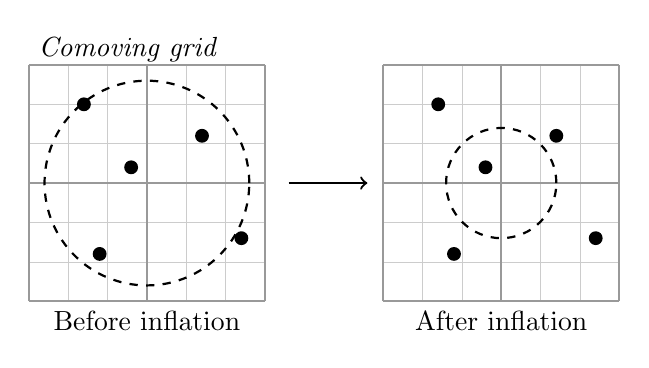
\begin{tikzpicture}
            \node[above, right] at (0,3.2) {\emph{Comoving grid}};
            % Fine grid
  \draw[step=0.5,gray!40,very thin] (0,0) grid (3,3);
  % Coarse grid
  \draw[step=1.5,gray!80,thick] (0,0) grid (3,3);

  % Scattered points
  \fill[black] (0.7,2.5) circle (2.5pt);
  \fill[black] (2.2,2.1) circle (2.5pt);
  \fill[black] (1.3,1.7) circle (2.5pt);
  \fill[black] (2.7,0.8) circle (2.5pt);
  \fill[black] (0.9,0.6) circle (2.5pt);

  % Large circle
  \draw[dashed, thick] (1.5,1.5) circle (1.3);
    % Fine grid
  \draw[step=0.5,gray!40,very thin] (4+.5,0) grid (7+.5,3);
  % Coarse grid
  \draw[step=1.5,gray!80,thick] (4+.4999,0) grid (7+.5,3);

  % Scattered points
  \fill[black] (4.7+.5,2.5) circle (2.5pt);
  \fill[black] (6.2+.5,2.1) circle (2.5pt);
  \fill[black] (5.3+.5,1.7) circle (2.5pt);
  \fill[black] (6.7+.5,0.8) circle (2.5pt);
  \fill[black] (4.9+.5,0.6) circle (2.5pt);

  % Large circle
  \draw[dashed, thick] (5.5+.5,1.5) circle (.7);
  \draw[->,thick] (3.3,1.5) -- (4+.3,1.5) ;
  \node[below] at (1.5,0) {Before inflation};
  \node[below] at (5.5+.5,0) {After inflation};
        \end{tikzpicture}
        \caption{Comoving Hubble horizon (dashed) before and after inflation.}
        \label{fig:shrinking_horizon}
    \end{subfigure}
    \begin{subfigure}[b]{0.5\textwidth}
        \centering
        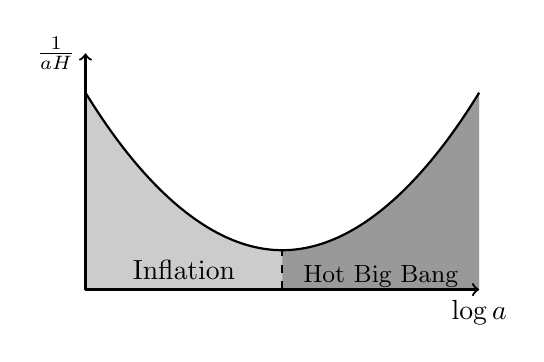
\begin{tikzpicture}
            \fill[black!20] (0,2.5) parabola bend (2.5,0.5) (5,2.5) -- (5,0) -- (0,0) -- cycle;
            \fill[black!40] (2.5,0.5) parabola bend (2.5,0.5) (5,2.5) -- (5,0) -- (2.5,0) -- cycle;
            \draw[->,thick] (0,0) -- (0,3) node[left] {$\frac{1}{aH}$};
            \draw[->,thick] (0,0) -- (5,0) node[below] {$\log a$};
            \draw[thick] (0,2.5) parabola bend (2.5,0.5) (5,2.5);
            \draw[dashed, thick] (2.5,0) -- (2.5,0.5);
            \node[above] at (3.75,-0.1) {\small{Hot Big Bang}};
            \node[above] at (1.25,0) {Inflation};
        \end{tikzpicture}
        \caption{Inflation contribution to the particle horizon.}
        \label{fig:inflation_contribution}
    \end{subfigure}
    \caption{Graphical representation of the ideas behind inflation. Figure (a) illustrates how the shrinking of the Hubble horizon separates points on the comoving grid. Figure (b) shows how inflation increases the total particle horizon, which corresponds to the shaded area under the graph of the comoving Hubble horizon.}
\end{figure}
\section{Slow-roll inflation}
We now know that a phase of accelerated expansion is required to solve the flatness problem, however we still don't know how this phase started and what kind of cosmic fluid drove it. At a first glance a vacuum dominated universe, which leads to de Sitter spacetime ($a(t)\propto e^{H_0t}$), could seem a candidate, however we must consider that inflation has to be a temporary phase which ends with the beginning of the radiation dominated era. A vacuum dominated universe, since the density of vacuum is constant while the density of matter and radiation decrease as the universe expands, would be eternal. We conclude that de Sitter spacetime is not the appropriate solution, and we should look for a cosmic fluid that resemble vacuum during inflation but that can also behave differently, ending the inflationary phase.

To determine whether inflation, within a determined model, is taking place the \textbf{first slow-roll parameter} $\epsilon_1$ is used: indeed we know that inflation occurs when the Hubble radius is shrinking, namely
\begin{equation}
    \label{eq:First_SR_paramteter}
    0>\frac{d}{dt}\frac{1}{aH}=-\frac{1}{a}\bigg[1+\frac{\dot H}{H^2}\bigg]\defeq-1+\epsilon_1,\qquad\Rightarrow\qquad\boxed{\epsilon_1\defeq-\frac{\dot H}{H^2}<1}.
\end{equation}
The main advantage of the first slow-roll parameter is that we can evaluate it in a specific model that we want to study and identify the conditions for its inflationary dynamics. Note that this parameter also quantifies the departure from de Sitter spacetime (since for de Sitter $H=$ const and thus $\epsilon_1=0$).

At this point we have to consider which cosmic fluid drives inflation: the easiest fluid, and yet complex enough to give rise to inflationary dynamics, is a scalar field, usually called \textbf{inflaton}. In general a scalar field $\phi(x)$ depends both on time and space, such scenario would spoil the symmetries of FRW metric and would require us to solve the full system of the Einstein equations coupled to the field. For this reason we assume that the field can be perturbatively expanded resulting in a background homogeneous field $\phi(t)$, plus some small perturbations $\delta \phi(t,\mathbf x)$, that can be later described in the context of a cosmological perturbation theory (Section \ref{sec:perturbations}) and will also have a quantum nature. In this way, the background  inflation field determines the dynamics of inflation, and it is treated completely classically, while its quantum perturbations will source anisotropies.\\
Starting from the action of the background inflaton field, with a generic potential, we can derive its equation of motion
\begin{equation}
    \mathcal{S}[\phi]=\int\ d^4x\sqrt{-g}\bigg(\frac{1}{2}\dot\phi^2(t)-V(\phi)\bigg)\qquad\Rightarrow\qquad\boxed{\ddot\phi+3H\dot \phi+\partial_\phi V(\phi)=0},\label{eq:motion_inflaton}
\end{equation}
and its energy-momentum tensor
\begin{equation}
   \tensor{T}{^\mu_\nu}=\partial^\mu\phi\partial_\nu\phi+\tensor{g}{^\mu_\nu}\mathcal{L}=
   \begin{cases}
    \tensor{T}{^0_0}=-\bigg(\frac{1}{2}\dot\phi^2(t)+V(\phi)\bigg)\\
    \tensor{T}{^i_j}=\bigg(\frac{1}{2}\dot\phi^2(t)-V(\phi)\bigg)\tensor{\delta}{^i_j}\\
   \end{cases}.
\end{equation}
By analogy with the energy-momentum tensor of a perfect fluid, we can compute the energy density ($\rho=-\tensor{T}{^0_0}$) and the pressure ($p=\tensor{T}{^i_i}/3$) associated to the inflaton field, which turn out to be respectively
\begin{equation}
    \label{eq_rho_p_inflaton}
    \rho=\frac{1}{2}\dot\phi^2(t)+V(\phi)\qquad\text{and}\qquad p=\frac{1}{2}\dot\phi^2(t)-V(\phi).
\end{equation}
By plugging the energy density of the inflaton in the Friedmann equation \eqref{eq:Friedmann1} we find
\begin{equation}
    H^2=\frac{8\pi G}{3}\bigg(\frac{1}{2}\dot\phi^2(t)+V(\phi)\bigg),
    \label{eq:Friedmann_inflaton}
\end{equation}
which should be solved to determine the evolution of the scale factor. However, at this stage we are not interested into the full dynamics of the scale factor and the inflaton, but we just want to understand the conditions for which it occurs. As we know the first slow-roll parameter can be exploited to this end
\begin{equation}
    \epsilon_1=-\frac{\dot H}{H^2}=\frac{\frac{3}{2}\dot\phi^2}{\big(\frac{1}{2}\dot\phi^2+V(\phi)\big)}=\frac{4\pi G\dot\phi^2}{H^2},\label{eq:SRP_field}
\end{equation}
where we obtained the time derivative of the Hubble parameter by differentiating the Friedmann equation \eqref{eq:Friedmann_inflaton} in which we inserted the equation of motion \eqref{eq:motion_inflaton}
$$2H\dot H=\frac{8\pi G}{3}\bigg(\dot\phi\ddot\phi+\partial_\phi V(\phi)\dot\phi\bigg)=-8\pi GH\dot \phi^2\quad\Rightarrow\quad \boxed{\dot H=-\frac{\dot \phi^2}{16\pi G}}.$$
Form the slow-roll parameter we immediately note that inflation occurs when $\dot \phi\ll V(\phi)$. Note that in this limit the inflaton field behaves as vacuum $$\omega\defeq\frac{p}{\rho}=\frac{\frac{1}{2}\dot\phi^2-V(\phi)}{\frac{1}{2}\dot\phi^2+V(\phi)}\xrightarrow{\dot\phi\ll V(\phi)}-1,$$
and thus, as we expect, we recover an approximated version of de Sitter spacetime.

The slow-roll condition is not the only requirement which we should make; indeed, if the inflaton field was to meet the condition $\epsilon_1<1$ for short time, inflation would end too soon. We therefore also require, to maintain inflationary conditions, that $\epsilon_1$ varies slowly: this is done by defining the \textbf{second slow-roll parameter}
\begin{equation}
    \epsilon_2\defeq\frac{\dot\epsilon_1}{H\epsilon_1}=2\frac{\ddot\phi}{\dot\phi H}-2\frac{\dot H}{H^2},\label{eq:second_sr_parameter}
\end{equation}
where we also computed its value for the scalar field model. This simple calculation shows that to maintain a slow-roll inflation also the condition $\ddot\phi\ll H\dot\phi$ should be satisfied. Indeed, imposing the above conditions, the equations of motion of the inflaton and of the scale factor reduce to
\begin{equation}
    \label{eq:SR_equation_motion}
    \dot\phi \approx-\frac{\partial_\phi V(\phi)}{3H},\qquad H^2\approx\frac{8\pi G}{3}V(\phi).
\end{equation}
These two equations shows that the dynamics of slow-roll inflation is fully determined by the potential of the inflaton. 
